\subsection*{Objective}
In Section \ref{RR}, some interesting results were obtained when attempting to run recursive refinement on an image with grapes in it.
Originally it was meant to see if individual grapes could be recognised.
On evaluation of the images used for training, it was found that bunches of grapes were used for training, not individual grapes. Therefore the results expected where never feasibly going to be obtained.
Even though this was the case, the script resulted in finding grapes in portions of the background, as seen in Figure \ref{fig:rr1}.
The purpose of this experiment is to look into why this is occurring.
A new image of a fruit bowl (Figure \ref{fig:fruitFromPhone}), taken on a mobile phone was selected for this experiment.
The image was used to run the script as defined in \ref{RR} but on two separate models.
The model with tuned parameters, trained on 108 classes, with a final test accuracy of 66.3\% and the model trained on 13 classes, with a final accuracy of 92.6\%.

\begin{figure}[h]
\centering
    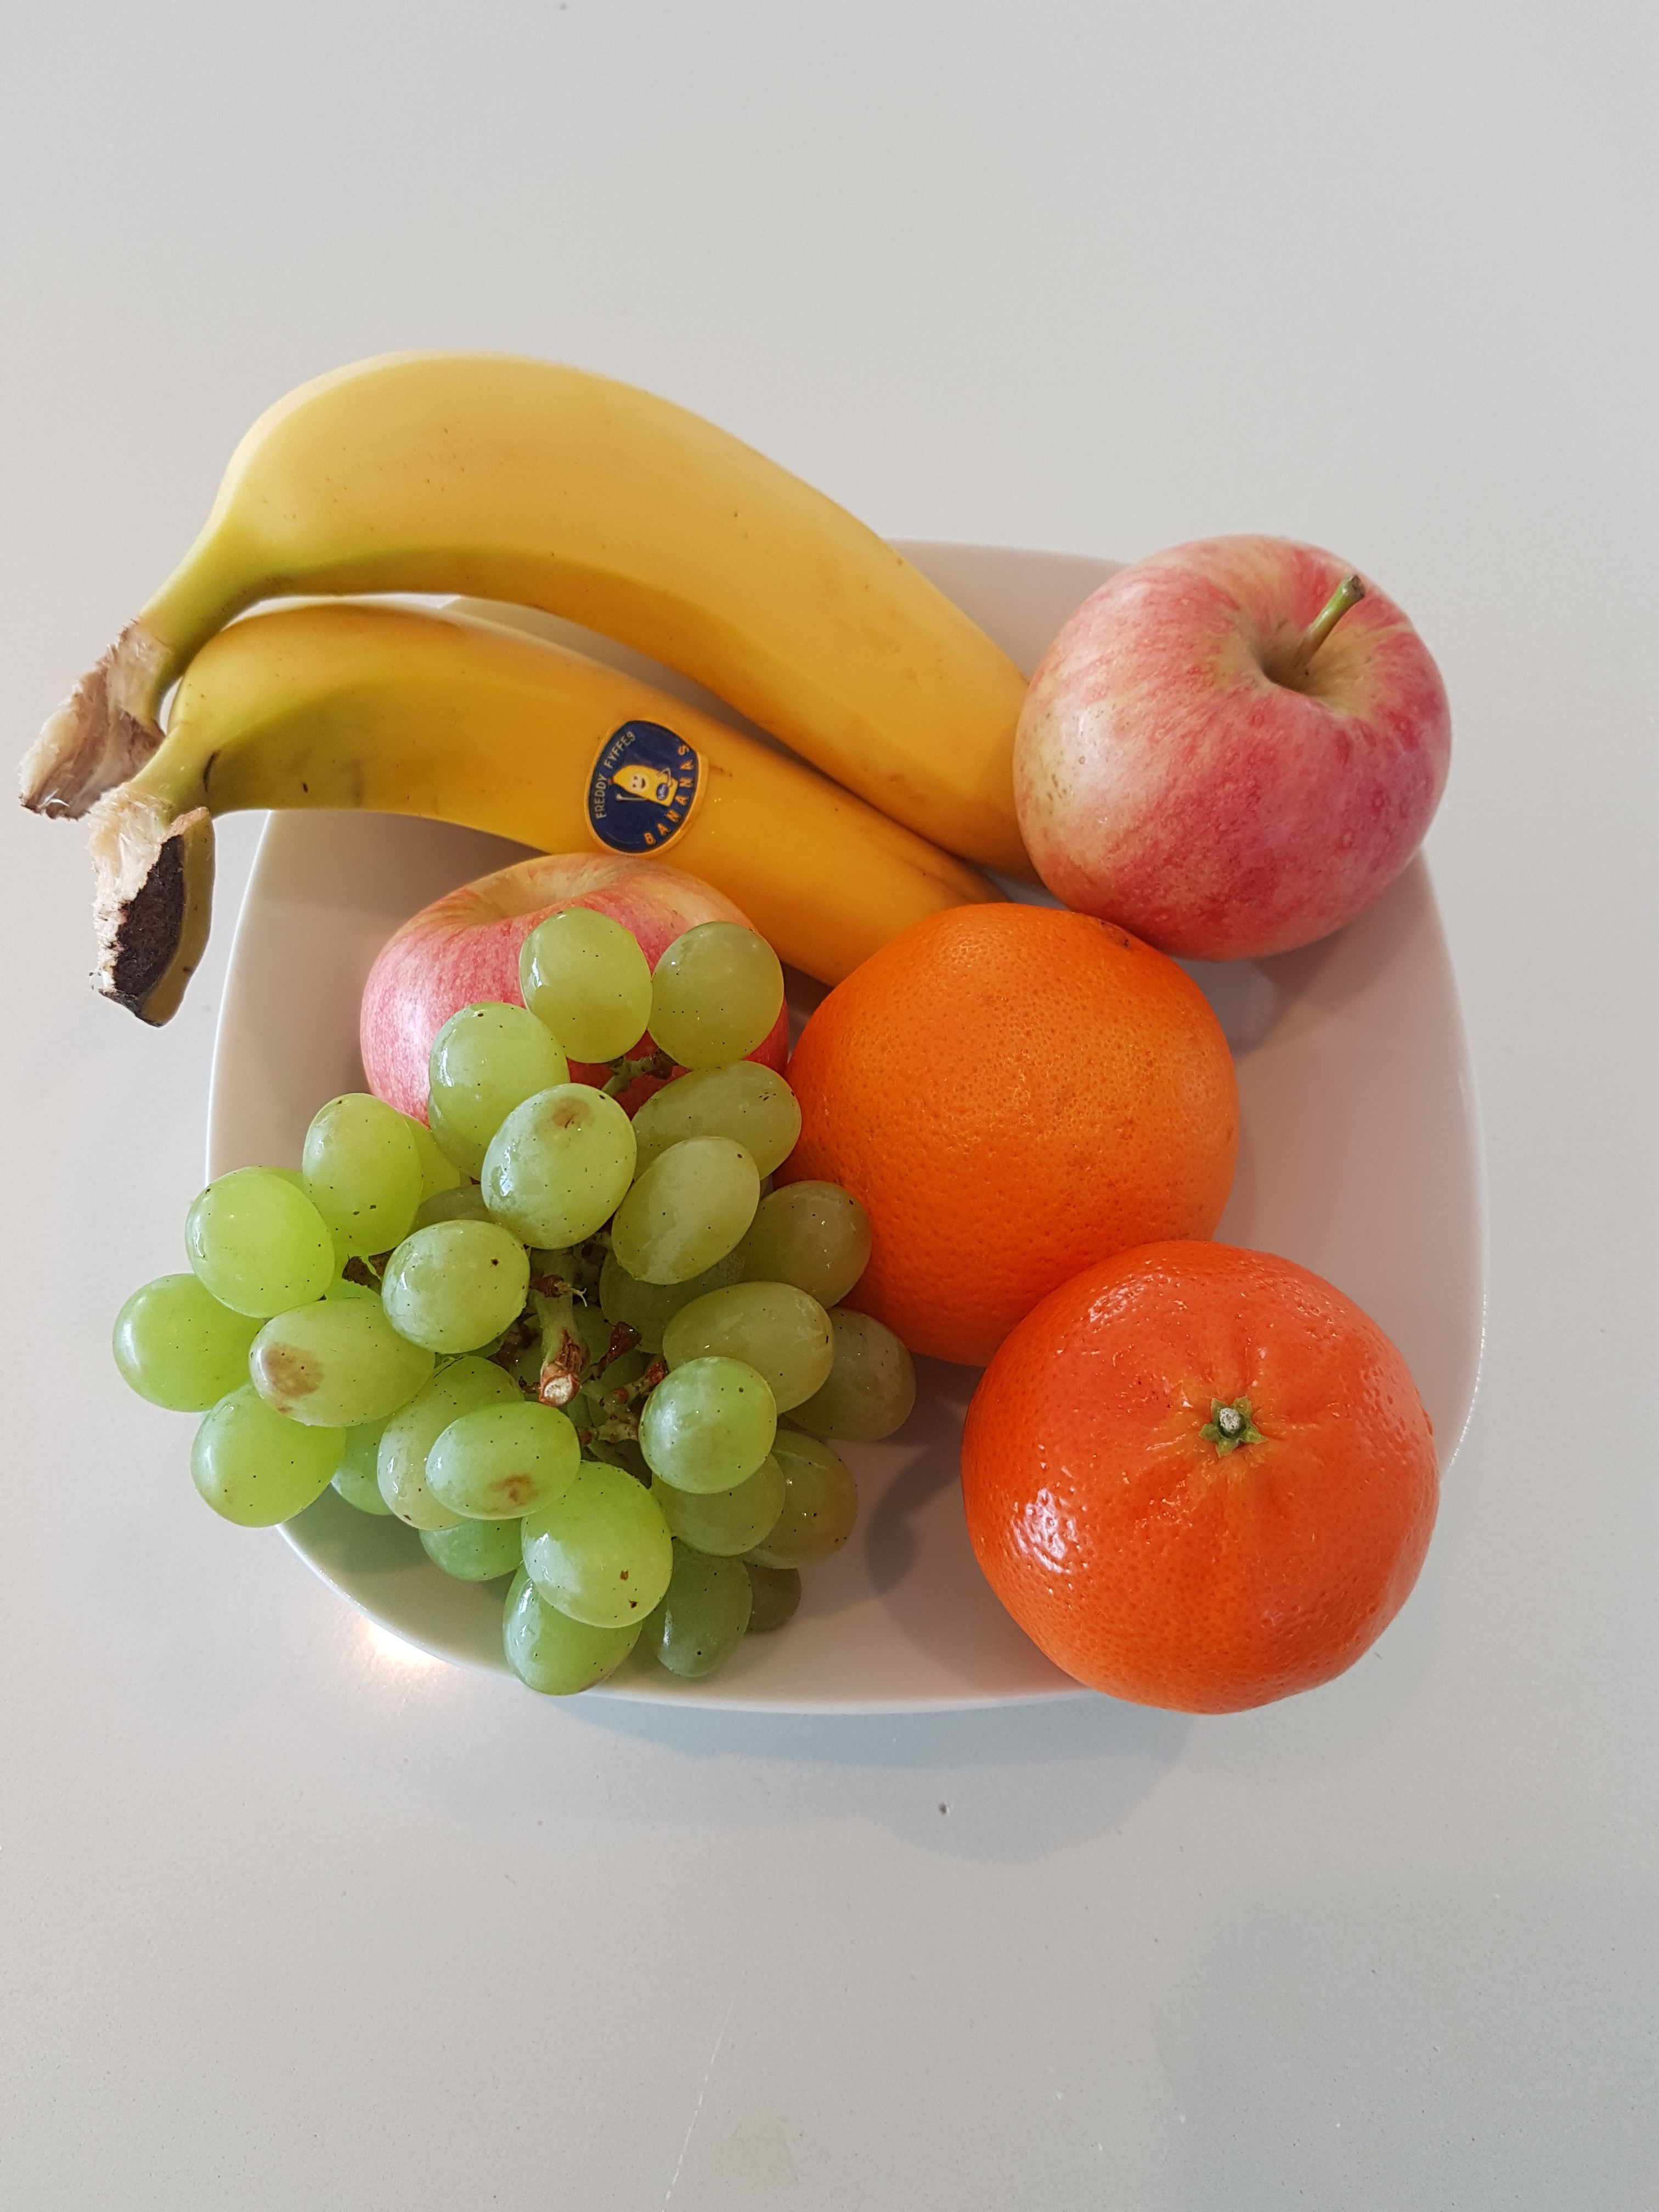
\includegraphics[scale=0.08]{fruitFromPhone}
      \caption{Fruit image taken on a mobile phone}
      \label{fig:fruitFromPhone}
\end{figure}

\subsection*{Results}
The outputs of the script can be seen in Figure \ref{fig:fruitRR13} and Figure \ref{fig:fruitRR108}. The output using the model trained on 13 classes had less false positive predictions. As the script ran (on both models), the segments predicted as grapes were saved to disk and then were each classified using 'label\_image.py'. The probabilities of the predictions were recorded with results as seen in Table \ref{RR_result_table}.

\begin{figure}[h]
\centering
    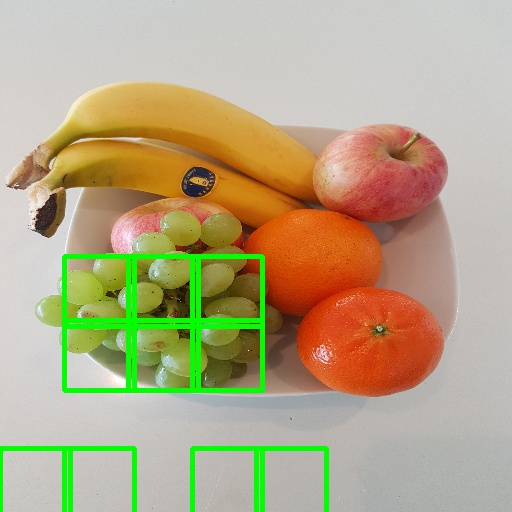
\includegraphics[scale=0.5]{fruitFromPhoneRR_13Classes}
      \caption{Image after sliding window - 13 classes}
      \label{fig:fruitRR13}
\end{figure}

\begin{figure}[h]
	\centering
    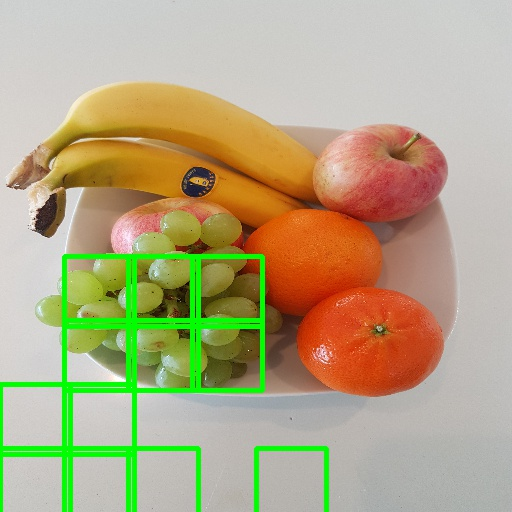
\includegraphics[scale=0.5]{fruitFromPhoneRR_108Classes}
      \caption{Image after sliding window - 108 classes}
      \label{fig:fruitRR108}
\end{figure}

\begin{table}[]
\centering
\caption{Results of recursive refinement segment classifications using two models}
\label{RR_result_table}
\begin{tabular}{|l|l|l|}
\hline
\textbf{Fruitbowl Segment} & \textbf{13 class model}                                                                                                                                       & \textbf{108 class model}                                                                                                                                   \\ \hline
False Positive 1                 & \begin{tabular}[c]{@{}l@{}}grape 0.31476045\\ apple 0.25866747\\ orange 0.11228518\\ apple pie 0.10234257\\ chocolate cake 0.09062083\end{tabular}   & \begin{tabular}[c]{@{}l@{}}grape 0.31820437\\ panna cotta 0.091400646\\ macarons 0.08560496\\ roll 0.08188102\\ apple 0.03981942\end{tabular}     \\ \hline
False Positive 2                 & \begin{tabular}[c]{@{}l@{}}grape 0.29391274\\ apple 0.2371384\\ orange 0.16196558\\ chocolate cake 0.10039616\\ apple pie 0.096121624\end{tabular}   & \begin{tabular}[c]{@{}l@{}}panna cotta 0.21783036\\ grape 0.105718106\\ apple 0.087030284\\ macarons 0.07753955\\ orange 0.037592527\end{tabular} \\ \hline
False Positive 3                 & \begin{tabular}[c]{@{}l@{}}grape 0.22402291\\ chocolate cake 0.16412543\\ apple 0.14523567\\ orange 0.12525927\\ apple pie 0.099948086\end{tabular}  & \begin{tabular}[c]{@{}l@{}}grape 0.2835378\\ panna cotta 0.088551655\\ macarons 0.06166248\\ orange 0.041896477\\ roll 0.040348493\end{tabular}   \\ \hline
False Positive 4                 & \begin{tabular}[c]{@{}l@{}}apple 0.37422368\\ grape 0.28592423\\ orange 0.10230055\\ chocolate cake 0.085367255\\ apple pie 0.053731006\end{tabular} & \begin{tabular}[c]{@{}l@{}}grape 0.20476209\\ macarons 0.17529227\\ panna cotta 0.16139281\\ roll 0.04359601\\ orange 0.036991216\end{tabular}    \\ \hline
False Positive 5                 & N/A                                                                                                                                                  & \begin{tabular}[c]{@{}l@{}}grape 0.22574392\\ macarons 0.14840269\\ panna cotta 0.08670294\\ roll 0.08650105\\ orange 0.046900786\end{tabular}    \\ \hline
False Positive 6                 & N/A                                                                                                                                                  & \begin{tabular}[c]{@{}l@{}}grape 0.31369162\\ panna cotta 0.11833602\\ macarons 0.09010604\\ apple 0.057512555\\ roll 0.047116004\end{tabular}    \\ \hline
\end{tabular}
\end{table}

\subsection*{Analysis}
\subsubsection*{Comparing the two models}
As we can see evidence of in Table \ref{RR_result_table}, along with Figure \ref{fig:fruitRR13} and Figure \ref{fig:fruitRR108}, the model trained on 13 classes predicted only four false positives while the larger model predicted 6.
This is most likely due to the larger model not being able to separate grapes as well as the smaller model.
It is worth mentioning that the grape class has the lowest number of training images of all the other classes.

\subsubsection*{Analysing Probabilities}
The probabilities of predictions for grapes in these false positive classifications are all low, in both models.
In contrast, some of the correctly classified segments were run through the model and the results all had probabilities in the high nineties.
When these background segments are run through the model, some prediction has to be made and none of these false predictions have a probability of over 0.4.
The average probability of these segments being grapes is in fact 0.257 (rounded to three decimal places).
A counter measure to this problem could be to disregard any predictions with a probability under a certain threshold, perhaps 0.4.

